% !TEX root = ../paper.tex
\section{GPU Optimizations}
\label{sec:optimizations}

This section details every GPU-level optimisation applied in the project,
with quantitative analysis of occupancy, bandwidth, and launch-overhead
trade-offs on Maxwell hardware (SM~5.0/5.3).

% ===================================================================
\subsection{Memory Coalescing via SoA Layout}
\label{sec:soa}

A warp of 32 threads issues a single memory transaction. With the
Structure-of-Arrays layout, threads 0--31 access contiguous floats and the
hardware merges the request into a single 128-byte transaction (100\%
efficiency). An Array-of-Structures layout would scatter accesses across
a stride equal to the struct size, wasting up to 90\% of bus bandwidth.

Indirect accesses introduced by the spatial grid
(\texttt{posX[particleIndex[s]]}) are not perfectly coalesced. However, after
CUB radix sort, particles within the same cell have nearby indices ---
loads are nearly coalesced and benefit from L2 cache reuse (the steady-state
working set of 4{,}000 particles fits in $\sim$128\,KB, or 12.5\% of the 1\,MB
L2 on the GTX~960M).

% ===================================================================
\subsection{Warp-Cooperative Shared-Memory Tiling}
\label{sec:tiling}

Shared memory is on-chip SRAM ($\sim$5-cycle latency, $\sim$1.3\,TB/s), compared
to global memory ($\sim$300--500 cycles, $\sim$30\,GB/s on Maxwell). The
\texttt{neighborCollisionKernel} employs \textbf{warp-cooperative tiling}: each
warp loads a tile of 32 neighbours into shared memory and all 32 threads read
from it. The tile is declared as \texttt{[MAX\_WARPS][WARP\_SIZE + 1]}, where
$\text{MAX\_WARPS} = 16 = 512/32$ and the \texttt{+1} padding avoids
shared-memory bank conflicts (successive warps access different banks):

\begin{lstlisting}
__shared__ float s_px[MAX_WARPS][WARP_SIZE+1];
__shared__ float s_py[MAX_WARPS][WARP_SIZE+1];
__shared__ float s_pz[MAX_WARPS][WARP_SIZE+1];
__shared__ float s_r [MAX_WARPS][WARP_SIZE+1];
__shared__ int   s_idx[MAX_WARPS][WARP_SIZE+1];
__shared__ int   s_state[MAX_WARPS][WARP_SIZE+1];
\end{lstlisting}

\textbf{Why \texttt{\_\_syncwarp()} instead of \texttt{\_\_syncthreads()}.}
The previous kernel used \texttt{\_\_syncthreads()} combined with symmetric
iteration. When excess threads executed an early \texttt{return} before the
barrier, the remaining threads deadlocked --- violating the CUDA specification
that \emph{all} threads in a block must reach the same
\texttt{\_\_syncthreads()}. The warp-scoped \texttt{\_\_syncwarp()} avoids this:
all 32 threads always participate in the tile load (the
\texttt{lane < tileLen} guard is a predicated branch, not an early return).

\textbf{Why velocities are not tiled.} Adding \texttt{s\_vx/vy/vz} would
increase per-block shared memory from $\sim$10.6\,KB to $\sim$17\,KB. At 3
resident blocks this exceeds the 48\,KB limit (51\,KB), reducing occupancy
from 75\% to 50\%. Velocities are instead loaded on-demand via
\texttt{\_\_ldg()} only when contact is detected, which is rare ($\sim$2--5
contacts out of 10--50 neighbours per cell).

% ===================================================================
\subsection{Atomic Reduction Strategy}
\label{sec:atomics}

On Maxwell, \texttt{atomicAdd} on FP32 generates a compare-and-swap (CAS) loop
that under contention executes 5--10 retry iterations. The previous symmetric
collision kernel (\texttt{j > i}) required 6~\texttt{atomicAdd} per pair.

The current design uses \textbf{full non-symmetric iteration}: every thread $i$
iterates over all neighbours $j \neq i$, accumulating forces entirely in
registers. The sole write is a direct store to
\texttt{forceX/Y/Z[i]} --- thread~$i$ is the only writer, so no atomic is
needed. This trades doubled FLOPs ($N$ vs.\ $N/2$ pair evaluations) for
\textbf{zero contention}, which is a net win on Maxwell where each CAS retry
costs 20--60 cycles versus $\sim$4 cycles for a direct store.

% ===================================================================
\subsection{Occupancy Tuning}
\label{sec:occupancy}

Occupancy is defined as the ratio of active warps to the maximum warps per SM
(64 on SM~5.0/5.3, i.e.\ 2048 threads). It is constrained by registers
(65{,}536/SM), shared memory (48\,KB/SM), and block count (max 32/SM).
Table~\ref{tab:occupancy} reports the per-kernel occupancy achieved.

\begin{table}[H]
  \caption{Per-kernel occupancy (\texttt{ptxas~-v} output).}
  \label{tab:occupancy}
  \centering
  \scriptsize
  \begin{tabular}{@{}lccccc@{}}
    \toprule
    \textbf{Kernel} & \textbf{Regs} & \textbf{Block} & \textbf{Blk/SM}
      & \textbf{Occ.} & \textbf{Limiter} \\
    \midrule
    \texttt{neighborCollision}    & 40 & 512 & 3 & 75.0\% & Shared mem. \\
    \texttt{forceTether}          & 27 & 256 & 8 & 100\%  & --- \\
    \texttt{integrateGround}      & 24 & 256 & 8 & 100\%  & --- \\
    \texttt{captureFromSnowpack}  & 48 & 256 & 5 & 62.5\% & Registers \\
    \texttt{shellPhysicsFused}    & 37 & 256 & 5 & 62.5\% & Registers \\
    \texttt{bruteForceCollision}  & 38 & 256 & 5 & 62.5\% & Registers \\
    \texttt{computeHash}          & 14 & 256 & 8 & 100\%  & --- \\
    \texttt{buildCellRanges}      &  7 & 256 & 8 & 100\%  & --- \\
    \texttt{clearPrevCells}       &  8 & 256 & 8 & 100\%  & --- \\
    \bottomrule
  \end{tabular}
\end{table}

All kernels report \textbf{zero register spill} in the \texttt{ptxas} output.
Four kernels operate below 100\%:

\begin{itemize}
  \item \textbf{\texttt{neighborCollision} (75\%)}: dual constraint --- 40
        regs $\times$ 512 $= 20{,}480$ regs/block ($\lfloor65536/20480\rfloor
        = 3$ blocks) and shared memory: $3 \times 12.4$\,KB $= 37$\,KB fits,
        but $4 \times 12.4$\,KB $= 49.6$\,KB exceeds 48\,KB.
  \item \textbf{\texttt{captureFromSnowpack} (62.5\%)}: 48 regs --- the
        highest in the project. The kernel computes \texttt{expf}, hash PRNG,
        3D distance, and quaternion rotation. Reaching 100\% would require 32
        regs (a 33\% cut), causing massive spill in a kernel that is already
        range-limited to $\sim$500--2{,}000 threads per frame.
  \item \textbf{\texttt{shellPhysicsFused} / \texttt{bruteForceCollision}
        (62.5\%)}: 37--38 regs + shared memory for brute-force tiling
        ($8 \times 257 \times 4$\,B $\approx 8$\,KB/block). At 6+ blocks
        shared memory exceeds budget. These kernels run only for
        $N \leq 2048$.
\end{itemize}

\textbf{Design principle: zero spill $>$ 100\% occupancy.} A single register
spill costs $\sim$300 cycles (DRAM round-trip), while one fewer warp costs
only a few scheduling cycles. For compute-bound kernels or kernels whose
working set fits in cache, keeping all variables in registers outweighs the
benefit of additional concurrent warps.

% ===================================================================
\subsection{Single Precision and Fast Math}
\label{sec:fp32}

Consumer Maxwell GPUs have an FP64\,:\,FP32 throughput ratio of 1\,:\,32.
With $\Delta t = 5$\,ms, the Euler truncation error
($O(\Delta t^2) \approx 2.5 \times 10^{-5}$) dominates FP32 rounding
($\epsilon \approx 6 \times 10^{-8}$) by three orders of magnitude, making
single precision entirely adequate. All literals are \texttt{f}-suffixed, all
math functions use \texttt{f}-variants (\texttt{sqrtf}, \texttt{expf},
\texttt{fmaxf}), and \texttt{M\_PI} is defined as \texttt{float}. The
\texttt{-{}-use\_fast\_math} flag enables fused operations and
flush-to-zero for denormals.

% ===================================================================
\subsection{\texttt{\_\_restrict\_\_} and \texttt{\_\_ldg()}}
\label{sec:ldg}

The \texttt{\_\_restrict\_\_} qualifier enables the compiler to reorder
loads/stores and cache values in registers. On SM $\geq$ 3.5,
\texttt{\_\_ldg()} routes loads through the read-only texture cache, which is
physically separate from the L1/shared memory used for read-write data. This
\textbf{doubles effective cache bandwidth} without conflicts. All physics and
grid kernels use explicit \texttt{\_\_ldg()} for immutable inputs; the capture
kernel uses \texttt{const \_\_restrict\_\_} pointers, which the compiler
auto-routes through the read-only cache at \texttt{-O3}.

% ===================================================================
\subsection{Constant Memory}
\label{sec:constant}

The \texttt{SimParams} struct ($\sim$152\,B) is placed in
\texttt{\_\_constant\_\_} memory. Its dedicated 64\,KB cache \textbf{broadcasts}
a single value to all 32 threads in a warp in $\sim$5 cycles, without consuming
registers. Physics constants (gravity, stiffness, damping, etc.) are read
identically by all threads --- a perfect broadcast use-case. The struct is
uploaded once at startup via \texttt{cudaMemcpyToSymbol}.

% ===================================================================
\subsection{Kernel Fusion}
\label{sec:fusion}

Two pairs of kernels were fused to eliminate global-memory round-trips:

\begin{itemize}
  \item \texttt{applyForces} + \texttt{shellCoreTether} $\to$
        \textbf{\texttt{forceTether}}: eliminates one round-trip for
        \texttt{forceX/Y/Z}.
  \item \texttt{integrate} + \texttt{groundCollision} $\to$
        \textbf{\texttt{integrateGround}}: eliminates one round-trip for
        position/velocity.
\end{itemize}

Fusion keeps intermediate results in registers rather than writing to global
memory and re-reading in a second kernel.

% ===================================================================
\subsection{Spatial Hashing and CUB Radix Sort}
\label{sec:spatial_hash}

Collision detection is reduced from $O(N^2)$ to $O(N \cdot k)$ via
uniform-grid spatial hashing~\cite{teschner2003}. The hash function uses
prime multiplication: $h = (c_x \cdot 73856093) \oplus (c_y \cdot 19349663)
\oplus (c_z \cdot 83492791)$ with additional bit-mixing, masked to a compact
table of size $\texttt{nextPowerOf2}(N \times 8)$. This reduces memory from
$\sim$75\,MB (full domain) to $\sim$256\,KB.

CUB \texttt{DeviceRadixSort::SortPairs} sorts (hash, particleIndex) pairs with
a pre-allocated temporary buffer and bit-count limited to
$\lceil\log_2(\text{tableSize})/4\rceil \times 4$ to minimise radix passes.
A \texttt{clearPrevCellsKernel} clears only cells used in the previous frame
(scatter-clear), avoiding a full-array \texttt{memset}.

% ===================================================================
\subsection{Sorted Snowpack and Binary-Search Capture}
\label{sec:binary_search}

The snowpack is static --- sorting it once at initialisation by \texttt{posX}
enables a host-side \texttt{std::lower\_bound}/\texttt{upper\_bound} each frame
to find the interval $[\text{lo}, \text{hi})$ within capture distance. The
kernel launches on this subset only, reducing threads from $10^6$ to
$\sim$500--2{,}000 (a 50--100$\times$ reduction). The host-side binary search
costs $\sim$1\,$\mu$s on the pinned sorted array.

% ===================================================================
\subsection{Mega-Fused Kernel for Small $N$}
\label{sec:mega_fused}

With $N \leq 2048$, the standard pipeline requires $\sim$10 GPU commands per
frame, adding $\sim$100--150\,$\mu$s of pure launch overhead on the GTX~960M
(each command incurs $\sim$10--15\,$\mu$s driver overhead). A single
\textbf{\texttt{shellPhysicsFusedKernel}} replaces the entire pipeline: gravity
$\to$ damping $\to$ tether $\to$ brute-force $O(N^2)$ collision $\to$ Euler
integration $\to$ ground collision. Forces \textbf{never transit through global
memory} --- they stay in registers throughout. At $N = 2048$, brute-force
collision is $4 \times 10^6$ iterations ($\sim$0.3\,ms), still well within
budget. Above 2048 the grid-based $O(N \cdot k)$ path becomes more efficient.

% ===================================================================
\subsection{Pinned Memory for Asynchronous Copies}
\label{sec:pinned}

Nsight Systems profiling revealed 30--40\,ms GPU stalls caused by
\texttt{cudaMemcpyAsync} targeting \textbf{pageable} host memory --- the driver
silently inserts a device-wide synchronisation. All host buffers for async
readback are now allocated with \texttt{cudaMallocHost} (pinned memory):
capture counters, sorted \texttt{posX}, and trace buffers. Additionally,
the capture count (int) and mass (float) are packed into a single 8-byte
buffer, reducing per-frame GPU commands from 4 to 2 ($\sim$20--30\,$\mu$s
saved).

% ===================================================================
\subsection{Multi-Stream Pipeline}
\label{sec:streams}

Physics and grid-build kernels run on dedicated non-blocking CUDA streams.
\texttt{simStream} executes forces $\to$ collision $\to$ integration;
\texttt{gridStream} builds the spatial hash in parallel with force computation.
An additional third \texttt{traceStream} handles asynchronous device-to-host 
copies for optional trace snapshots. Fork/join is implemented via
\texttt{cudaEventRecord}/\texttt{cudaStreamWaitEvent} with timing-disabled
events to minimise overhead.

\begin{figure}[H]
  \centering
  \fbox{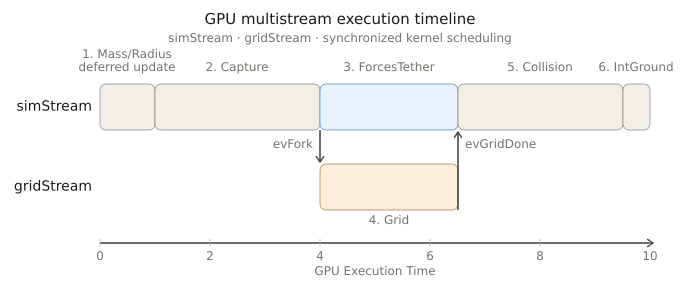
\includegraphics[width=0.9\columnwidth]{figures/multistream.png}}
  \caption{Dual-stream pipeline. Stages~3 and~4 overlap on separate streams;
  stage~5 waits for both via a lightweight CUDA event.}
  \label{fig:pipeline}
\end{figure}

% ===================================================================
\subsection{Gated Event Recording}
\label{sec:gated_events}

Each \texttt{cudaEventRecord()} call incurs $\sim$10--15\,$\mu$s driver
overhead. With up to 14 event records per frame (start\,+\,end for 7
timing pairs), this adds $\sim$110--165\,$\mu$s per frame. Events are recorded
only every \texttt{TIMING\_INTERVAL\,=\,64} frames (or when logging/rendering
is active). The 63~non-profiled frames save $\sim$12 event records each.
Synchronisation events (\texttt{evFork}, \texttt{evGridDone}) are always
recorded since they are required for correctness.

% ===================================================================
\subsection{ALU Optimizations}
\label{sec:alu}

\begin{itemize}
  \item \textbf{\texttt{rsqrtf} pattern}: $1/\sqrt{x}$ in a single SFU cycle
        ($\sim$8 cycles), then \texttt{dist = dist2 * invDist} (1 FMA), saving
        one SFU op compared to \texttt{sqrtf + 1.0f/dist}.
  \item \textbf{Tangential friction}: squared-magnitude threshold
        (\texttt{vt2 > 1e-16f}) with \texttt{rsqrtf(vt2)} avoids a separate
        \texttt{sqrtf} + division.
  \item \textbf{Branchless clamping}: \texttt{fmaxf(f\_spring - f\_damp, 0.0f)}
        compiles to a single \texttt{FMNMX} instruction (1~cycle) on Maxwell.
  \item \textbf{Hash-based PRNG}: a murmurhash variant (6 integer ops) replaces
        \texttt{curand} in the capture kernel, eliminating 48\,B/thread of
        global-memory state.
  \item \textbf{Quaternion rotation}: the Rodrigues formula uses 15 FMA
        operations versus 27 for a 3$\times$3 matrix multiply, and avoids
        constructing a temporary matrix (9 registers).
\end{itemize}

% ===================================================================
\subsection{Unity Build and Constant Sharing}
\label{sec:unity}

All GPU source files (\texttt{grid.cu}, \texttt{simulation.cu},
\texttt{snowpack.cu}) are \texttt{\#include}d into a single translation unit
\texttt{gpu\_unity.cu}. This shares the \texttt{\_\_constant\_\_ SimParams
d\_params} declaration across all kernels without separate compilation,
avoiding device-link overhead.

% ===================================================================
\subsection{Memory Hierarchy Summary}
\label{sec:mem_hierarchy}

Table~\ref{tab:mem_hierarchy} summarises how each memory level is exploited.

\begin{table}[H]
  \caption{Memory hierarchy utilisation.}
  \label{tab:mem_hierarchy}
  \centering
  \scriptsize
  \begin{tabular}{@{}lll@{}}
    \toprule
    \textbf{Level} & \textbf{Usage} & \textbf{Size} \\
    \midrule
    Registers        & Local vars, force accumulators & 24--48/thread \\
    \texttt{\_\_constant\_\_} & \texttt{SimParams} (broadcast) & $\sim$152\,B \\
    Shared memory    & Warp-cooperative tile          & 12.4\,KB/blk \\
    Read-only cache  & \texttt{\_\_ldg()} loads (immutable SoA fields)        & HW-managed \\
    L2 cache         & Particle working set           & 1\,MB / 256\,KB \\
    Global (GDDR5)   & SoA arrays                     & $16N \times 4$\,B \\
    \bottomrule
  \end{tabular}
\end{table}

\subsection{Holistic Optimization Strategy}
\label{sec:holistic}

The optimizations described above are not applied independently, but as an
integrated strategy responding to Maxwell's specific constraints. Register
pressure is minimized through constant memory (broadcasts), tiling (shared-memory
reuse), and fusion (avoiding intermediate global writes). This architecture-aware
methodology ensures that every optimization decision is motivated by profiling data
and hardware-specific trade-offs, rather than generic best practices.
